%%
%% Copyright 2007, 2008, 2009 Elsevier Ltd
%%
%% This file is part of the 'Elsarticle Bundle'.
%% ---------------------------------------------
%%
%% It may be distributed under the conditions of the LaTeX Project Public
%% License, either version 1.2 of this license or (at your option) any
%% later version.  The latest version of this license is in
%%    http://www.latex-project.org/lppl.txt
%% and version 1.2 or later is part of all distributions of LaTeX
%% version 1999/12/01 or later.
%%
%% The list of all files belonging to the 'Elsarticle Bundle' is
%% given in the file `manifest.txt'.
%%

%% Template article for Elsevier's document class `elsarticle'
%% with numbered style bibliographic references
%% SP 2008/03/01
%%
%%
%%
%% $Id: elsarticle-template-num.tex 4 2009-10-24 08:22:58Z rishi $
%%
%%
%%\documentclass[preprint,12pt]{elsarticle}

%% Use the option review to obtain double line spacing
%% \documentclass[preprint,review,12pt]{elsarticle}

%% Use the options 1p,twocolumn; 3p; 3p,twocolumn; 5p; or 5p,twocolumn
%% for a journal layout:
%% \documentclass[final,1p,times]{elsarticle}
%% \documentclass[final,1p,times,twocolumn]{elsarticle}
%% \documentclass[final,3p,times]{elsarticle}
 \documentclass[preprint,3p,times,twocolumn]{elsarticle}
%% \documentclass[final,5p,times]{elsarticle}
%%\documentclass[final,5p,times,twocolumn]{elsarticle}

%% if you use PostScript figures in your article
%% use the graphics package for simple commands
 \usepackage{graphics}
%% or use the graphicx package for more complicated commands
%% \usepackage{graphicx}
%% or use the epsfig package if you prefer to use the old commands
%% \usepackage{epsfig}

%% The amssymb package provides various useful mathematical symbols
\usepackage{amssymb}
%% The amsthm package provides extended theorem environments
%% \usepackage{amsthm}

%% The lineno packages adds line numbers. Start line numbering with
%% \begin{linenumbers}, end it with \end{linenumbers}. Or switch it on
%% for the whole article with \linenumbers after \end{frontmatter}.
%% \usepackage{lineno}

%% natbib.sty is loaded by default. However, natbib options can be
%% provided with \biboptions{...} command. Following options are
%% valid:

%%   round  -  round parentheses are used (default)
%%   square -  square brackets are used   [option]
%%   curly  -  curly braces are used      {option}
%%   angle  -  angle brackets are used    <option>
%%   semicolon  -  multiple citations separated by semi-colon
%%   colon  - same as semicolon, an earlier confusion
%%   comma  -  separated by comma
%%   numbers-  selects numerical citations
%%   super  -  numerical citations as superscripts
%%   sort   -  sorts multiple citations according to order in ref. list
%%   sort&compress   -  like sort, but also compresses numerical citations
%%   compress - compresses without sorting
%%
%% \biboptions{comma,round}

% \biboptions{}


\journal{Journal of Parallel and Distributed Computing}

\begin{document}

\begin{frontmatter}

%% Title, authors and addresses

%% use the tnoteref command within \title for footnotes;
%% use the tnotetext command for the associated footnote;
%% use the fnref command within \author or \address for footnotes;
%% use the fntext command for the associated footnote;
%% use the corref command within \author for corresponding author footnotes;
%% use the cortext command for the associated footnote;
%% use the ead command for the email address,
%% and the form \ead[url] for the home page:
%%
%% \title{Title\tnoteref{label1}}
%% \tnotetext[label1]{}
%% \author{Name\corref{cor1}\fnref{label2}}
%% \ead{email address}
%% \ead[url]{home page}
%% \fntext[label2]{}
%% \cortext[cor1]{}
%% \address{Address\fnref{label3}}
%% \fntext[label3]{}

\title{Hybrid Parallel Programming for Blue Gene/P}

%% use optional labels to link authors explicitly to addresses:
%% \author[label1,label2]{<author name>}
%% \address[label1]{<address>}
%% \address[label2]{<address>}

\author{Mads Ruben Burgdorff Kristensen}
\author{Hans Henrik Happe}
\author{Brian Vinter}
\address{eScience Center - University of Copenhagen Denmark}

\begin{abstract}
The concept of massively parallel processors has been taken to the extreme with the introduction of the BlueGene architectures from IBM. With hundreds of thousands of processors in one machine the parallelism is extreme, but so are the techniques that must be applied to obtain performance with that many processors. 
In this work we present optimizations of a Grid-based projector-augmented wave method software, GPAW \cite{Mortensen05} for the Blue Gene/P architecture. The improvements are achieved by exploring the advantage of shared and distributed memory programming also known as hybrid programming. The work focuses on optimizing a very time consuming operation in GPAW, the stencil operation, and different hybrid programming approaches are evaluated. The work succeeds in demonstrating a hybrid programming model which is clearly beneficial compared to the original flat programming model. In total an improvement of 1.94 compared to the original implementation is obtained. The results we demonstrate here are reasonably general and may be applied to other stencil codes.
\end{abstract}

\begin{keyword}
%% keywords here, in the form: keyword \sep keyword
GPAW \sep HPC \sep Hybrid-programming \sep multicore platforms

%% MSC codes here, in the form: \MSC code \sep code
%% or \MSC[2008] code \sep code (2000 is the default)

\end{keyword}

\end{frontmatter}

%%
%% Start line numbering here if you want
%%
% \linenumbers

\section{Introduction}
Grid Based Projector Augmented Wave (GPAW)\cite{Mortensen05} is a simulation software, which simulates many-body systems at the sub-atomic level. GPAW is primarily used by physicists and chemists to investigate the electronic structure, principally the ground state, of many-body systems. A significant part of a GPAW computation consists of a distributed stencil operation. The main object of this paper is to optimize this stencil operation on the Blue Gene/P\cite{BGPoverview} (BGP).

The current trend in HPC hardware is towards systems of shared-memory computation nodes. The BGP also follows this trend and consists of four CPU-cores per node. Furthermore it is quite possible that future versions of the Blue Gene architecture will consists of even more CPU-cores per node.

To exploit the memory locality in shared-memory computation nodes a paradigm which combines shared and distributed memory programming may be of interest. The idea is to avoid communication between CPU-cores on the same node. Unfortunately, it is not trivial to obtain good performance when combining shared-memory programming with distributed memory programming. Even though inter-CPU communication is avoided, it is often the case that the sole use of MPI\cite{mpi} outperforms a combination of threads and MPI when computing on clusters of shared-memory computation nodes\cite{henty2000, hipp04Hybrid, VinterB}.

We evaluate two different hybrid programming approaches. One approach in which inter-node communication is handled individually by every thread and another approach in which one thread handles the inter-node communication on behalf of all the other threads in a node. The work shows that, on the Blue Gene/P, the first approach is clearly superior the latter. In \cite{Cappello2000} the authors concludes that, on a well balanced system, a loop level parallelization approach, corresponding to our second hybrid approach, is unfavorably compared to a strictly MPI implementation. Our first hybrid approach was developed on the basis of that conclusion.

\section{GPAW}
GPAW is a real-space grid implementation of the projector augmented wave method\cite{paw}. It uses uniform real-space grids and the finite-difference approximation for the density functional theory calculations.

A central part of density functional theory and a very time consuming task in GPAW, is to solve Poisson and Kohn-Sham equations. Both equations rely on stencil operations when solved by GPAW. When solving the Poisson equation, a stencil is applied to the electrostatic potential of the system. When solving the Kohn-Sham equation, a stencil is applied to all wave-functions in the system. Both the electron density and the wave-functions are represented by real-space grids. A system typically consists of one electron density and thousands of wave-functions. The number of wave-functions in a system depends on the number of valence electrons in the system. For every valence electron there may be up to two wave-functions.

The computational magnitude of a GPAW simulation depends mainly on three factors: The world size, simulation system resolution and the number of valence electrons. The world size and resolution determine the dimensions of the real-space grids and the number of valence electrons determines the number of real-space grids.

A user is typically more interested in adding valence electrons to the simulation than to increase the size or resolution of the world. The real-space grid size will ordinary be between $100^3$ to $200^3$ where as the total number of real-space grids will be greater than thousand.

\subsection{Stencil Operation}
\begin{figure}
 \centering
 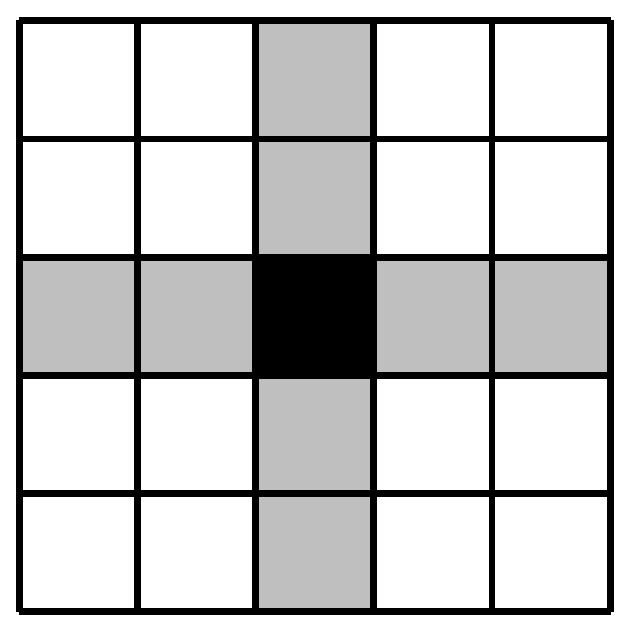
\includegraphics[width=45px]{gfx/stencil}
 \caption{A stencil operation on a 2D grid.}
 \label{fig:stencil}
\end{figure}
A stencil operation updates a point in a grid based on the surrounding points. A typical 2D example is illustrated in Figure \ref{fig:stencil} where points are updated based on the two nearest points in all four directions.

Stencil operations on the real-space grids (3D arrays) are used for the finite-difference approximation in GPAW. The stencil operation used is a linear combination of a point's two nearest neighbors in all six directions and itself. 
The stencil operations do normally use periodic boundary condition but that is not always the case.

If we look at the real-space grid $A$ and a predefined list of constants $C$, a point $A_{x,y,z}$ is computed like this:
\begin{displaymath}
\begin{array}{ll}
A'_{x,y,z} &= C_1 A_{x,y,z} + C_2 A_{x-1,y,z} + C_3 A_{x+1,y,z} +\\
           &  C_4 A_{x-2,y,z} + C_5 A_{x+2,y,z} + C_6 A_{x,y-1,z} +\\
           &  C_7 A_{x,y+1,z} + C_8 A_{x,y-2,z} + C_9 A_{x,y+2,z} +\\
           &  C_{10} A_{x,y,z-1} + C_{11} A_{x,y,z+1} +\\
           &  C_{12} A_{x,y,z-2} + C_{13} A_{x,y,z+2}\\
\end{array}
\end{displaymath}

\section{Blue Gene/P}
% An example of a floating table. Note that, for IEEE style tables, the 
% \caption command should come BEFORE the table. Table text will default to
% \footnotesize as IEEE normally uses this smaller font for tables.
% The \label must come after \caption as always.
%
\begin{table}
%% increase table row spacing, adjust to taste
%\renewcommand{\arraystretch}{1.3}
% if using array.sty, it might be a good idea to tweak the value of
% \extrarowheight as needed to properly center the text within the cells
\caption{Hardware description of a Blue Gene/P node}
\label{tab:bgp}
\centering
%% Some packages, such as MDW tools, offer better commands for making tables
%% than the plain LaTeX2e tabular which is used here.
\begin{footnotesize}
\begin{tabular}{l l}
\hline
Node CPU & Four PowerPC 450 cores\\
CPU frequency & 850 MHz\\
L1 cache (private) & 64KB per core\\
L2 cache (private) & Seven stream pre\-fetching\\
L3 cache (shared) & 8MB\\
Main memory & 2GB\\
Main memory bandwidth & 13.6GB/s\\
Peak performance & 13.6 Gflops/node\\
Torus bandwidth & 6 $\times$ 2 $\times$ 425MB/s = 5.1GB/s\\
\hline
\end{tabular}
\end{footnotesize}
\end{table}

Blue Gene/P consists of a number of nodes interconnected with three independent networks: a 3D torus network, a collective tree structured network, and a global barrier network. All point-to-point communication goes through the torus network and every node is equipped with a direct memory access (DMA) engine to offload torus communication from the CPUs. The collective tree structured network is used for collective operation like the MPI \emph{reduce} operation and the global barrier network is used for barriers.

Table \ref{tab:bgp} is a brief description of a BGP node. One thing to highlight is the ratio between the speed of the CPU-cores and the main memory. 
Since the CPU-cores are relatively slow and the main memory is relatively fast compared to today's standard, the performance of the main memory is not as far behind the CPU as usually. Furthermore, the torus bandwidth is only three times lower than the main memory if all six connections are used. The von Neumann bottleneck associated with main memory and network is therefore reduced.

The CPU-cores can be utilized by normal SMP approaches like pthread or OpenMP, with the limitation that BGP only supports one thread per CPU-core. The BGP addresses the problem of utilizing multiple CPU-cores by supporting a virtual partition of the nodes. From the programmers point of view the four CPU-cores would then look like four individual nodes with each 512MB of main memory. This virtual partitioning is called virtual mode.

\subsection{MPI}
BGP implements the MPICH2 library which comply with the MPI-2 specification\cite{mpi2}. MPI-2 specifies different levels of threaded communication. BGP supports the fully thread-safe mode called \texttt{MULTIPLE} which allows any thread to call the MPI library at any time. Since there is an overhead associated with \texttt{MULTIPLE} (e.g. locks), it is also possible to use the more restricted \texttt{SINGLE} mode, which do not allow concurrent calls to MPI.

The MPICH2 implementation is tailored to utilize the BGP's DMA engine which means that non-block\-ing MPI communication is handled asynchronously with minimum CPU involvement.

BGP supports the \texttt{MPI\_Cart\_create} function which tells BGP to reorder the MPI ranks in order to match the torus network. We make use of this function in all the following.

\begin{figure}
 \centering
 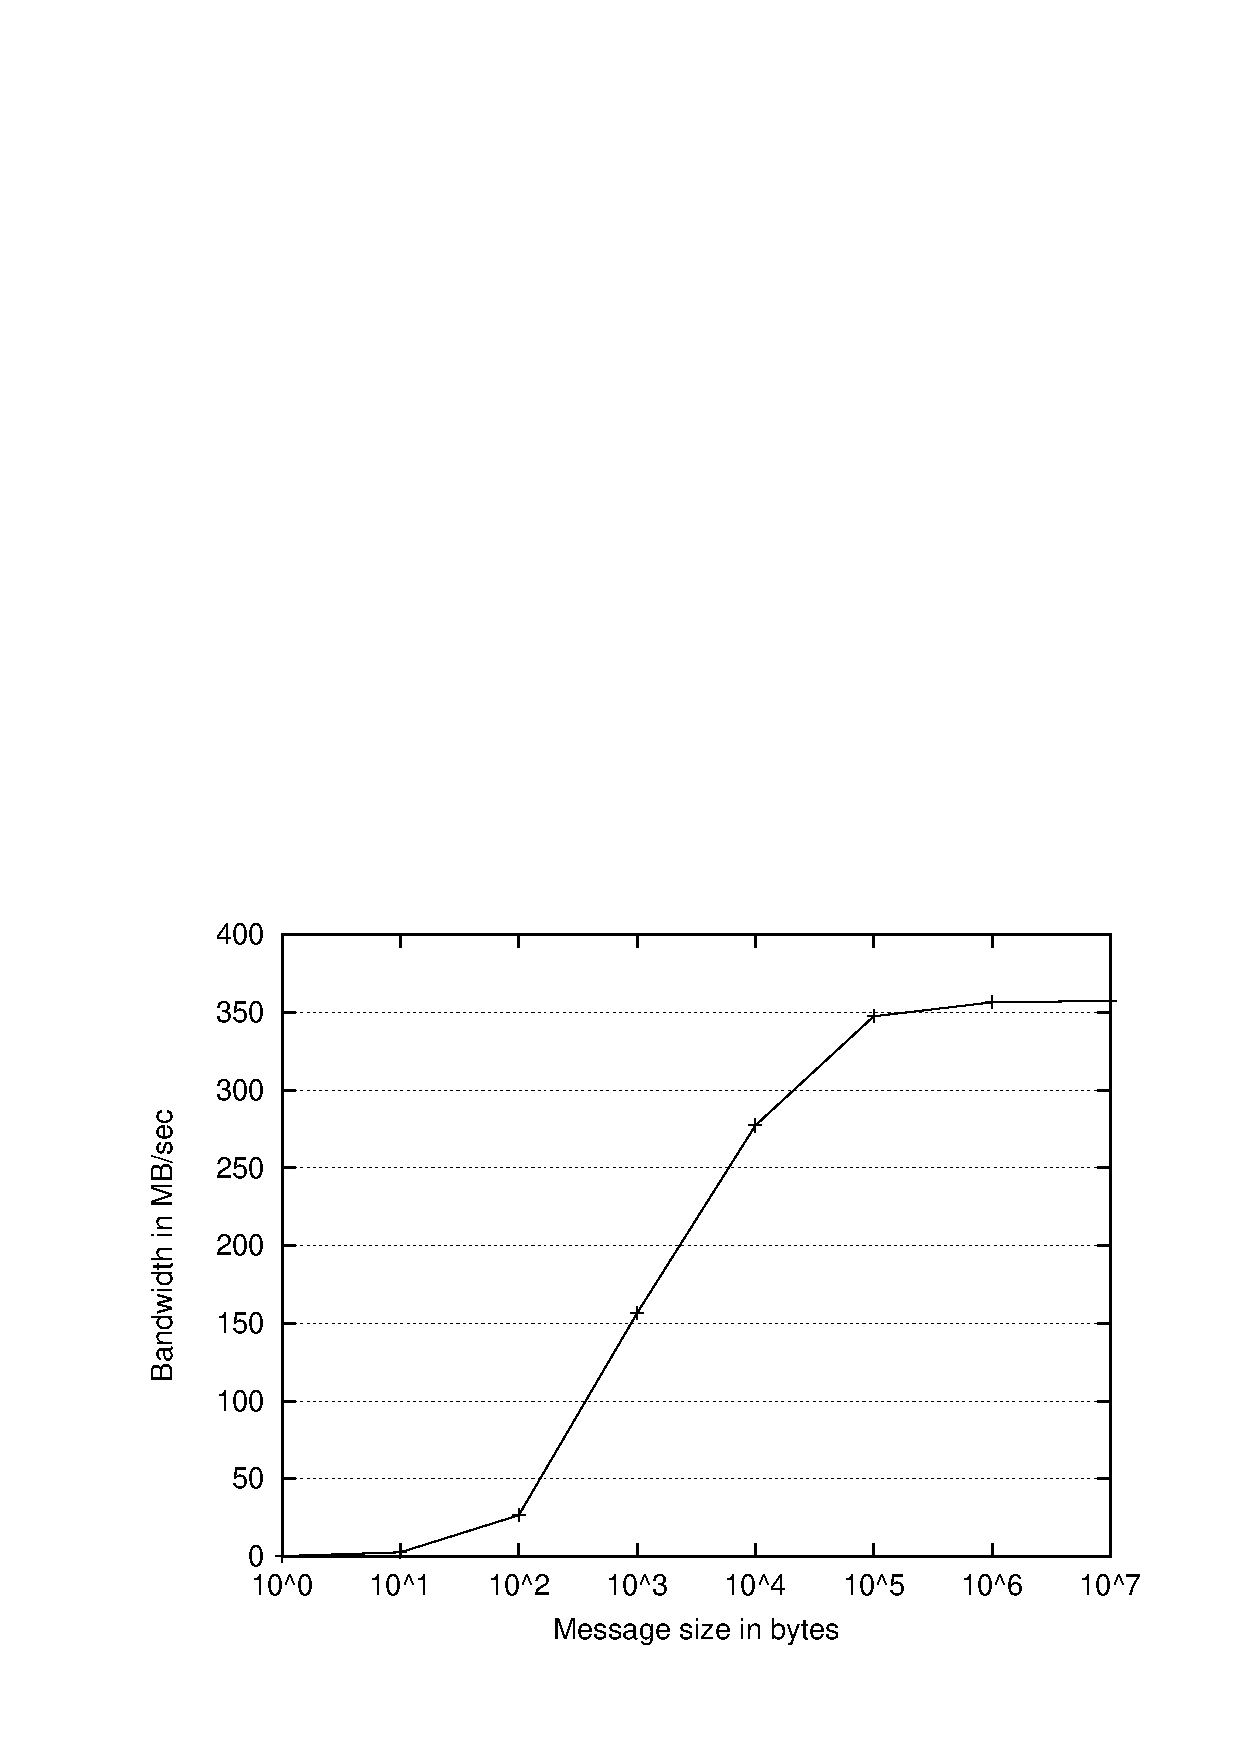
\includegraphics[width=\linewidth]{gfx/bgp_batchsize}
 \caption{A bandwidth graph showing how the message size influence the bandwidth. In this experiment, one MPI message is send between two neighboring BGP nodes.}
 \label{fig:batchsize}
\end{figure}

To investigate how much the message size influence point-to-point bandwidth, we have performed an experiment in which one MPI message is send between two neighboring BGP nodes (Figure \ref{fig:batchsize}). The result of the experiment clearly shows that in order to maximize the bandwidth, a message size greater than $10^5$ bytes is needed, while half the asymptotic bandwidth is achieved at approximate $10^3$ bytes.


\section{The GPAW implementation}\label{section:GPAW_impl}
\begin{figure}
 \centering
 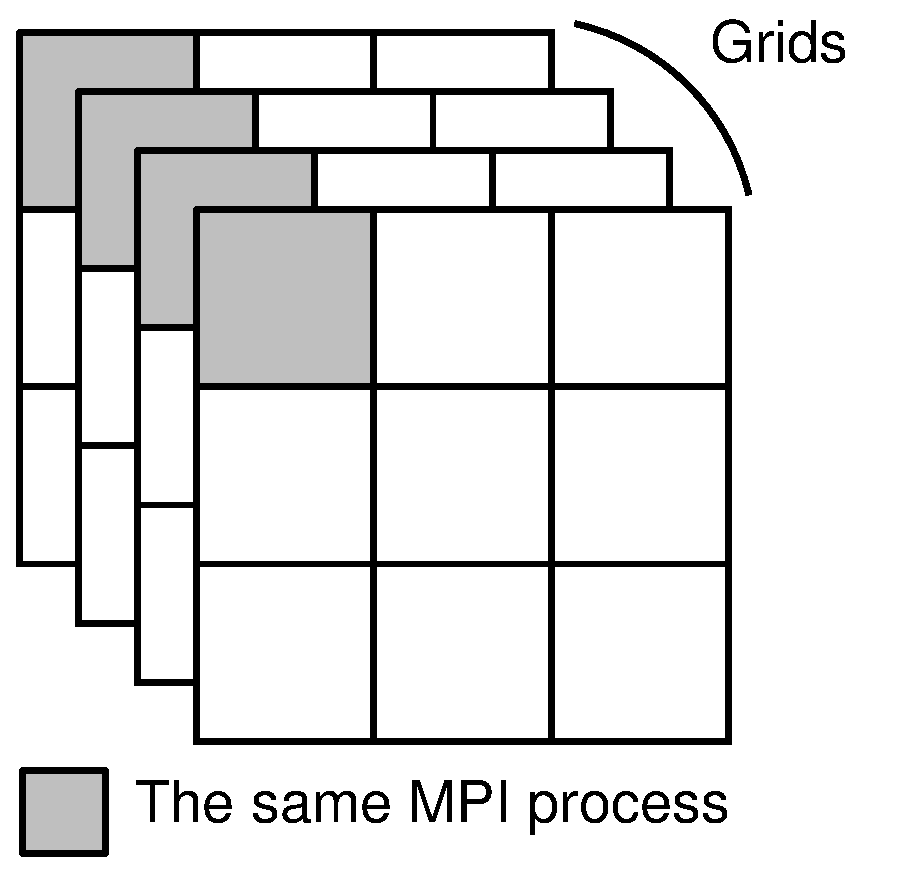
\includegraphics[width=100px]{gfx/wavedist}
 \caption{Four 2D grids distributed over nine processes.}
 \label{fig:wavedist}
\end{figure}

GPAW is implemented using C and Python. The intention is that the users of GPAW should write the model description in Python and then call C and Fortran functions from within Python. It is in this context a user would apply the C implemented stencil operation on one or more real-space grids.

The parallel version of GPAW uses MPI in a flat programming model and the parallelization is done by simple domain decomposition of every real-space grid in the simulation. That is, every MPI process gets the same subset of \emph{every} real-space grid in the simulation. This is important because some part of the GPAW computation, like the orthogonalization of wave-functions, requires the same subset of every real-space grid in the simulation. This is illustrated in Figure \ref{fig:wavedist} with 2D real-space grids instead of 3D grids.

The grids are simply divided into a number of quadrilaterals matching the number of available MPI processes. If no user-defined domain decomposition is present, GPAW will try to minimize the aggregated surface of the quadrilaterals. A real-space grid is represented as a three dimensional array where every point in the grid can be a real or complex number (8 or 16 bytes)

\subsection{Distributed Stencil Operation}
Generally, it should be easy to obtain good scalability for a distributed stencil operation since computation grows faster than communication. If we look at a 3D grid of size $n \times n \times n$ the aggregated computation is $O\left(n^3\right)$ where as the aggregated communication is only $O\left(n^2\right)$. The operation should scale very well when $n$ grows at the same rate as the number of CPUs.

In GPAW, however, scalability is very hard to obtain since the grid size will ordinarily not exceed $200^3$. Furthermore, since GPAW requires that every MPI process gets the same subset of every grid, it is hard to take advantage of the fact that the number of grids grows at the same pace as the CPUs.

One feature in GPAW, which makes it easier to parallelize, is the fact that the input grid and the output grid used in the stencil operation is always two separate grids. We need therefore not consider the order in which the grid-points are computed.

\begin{figure}
 \centering
 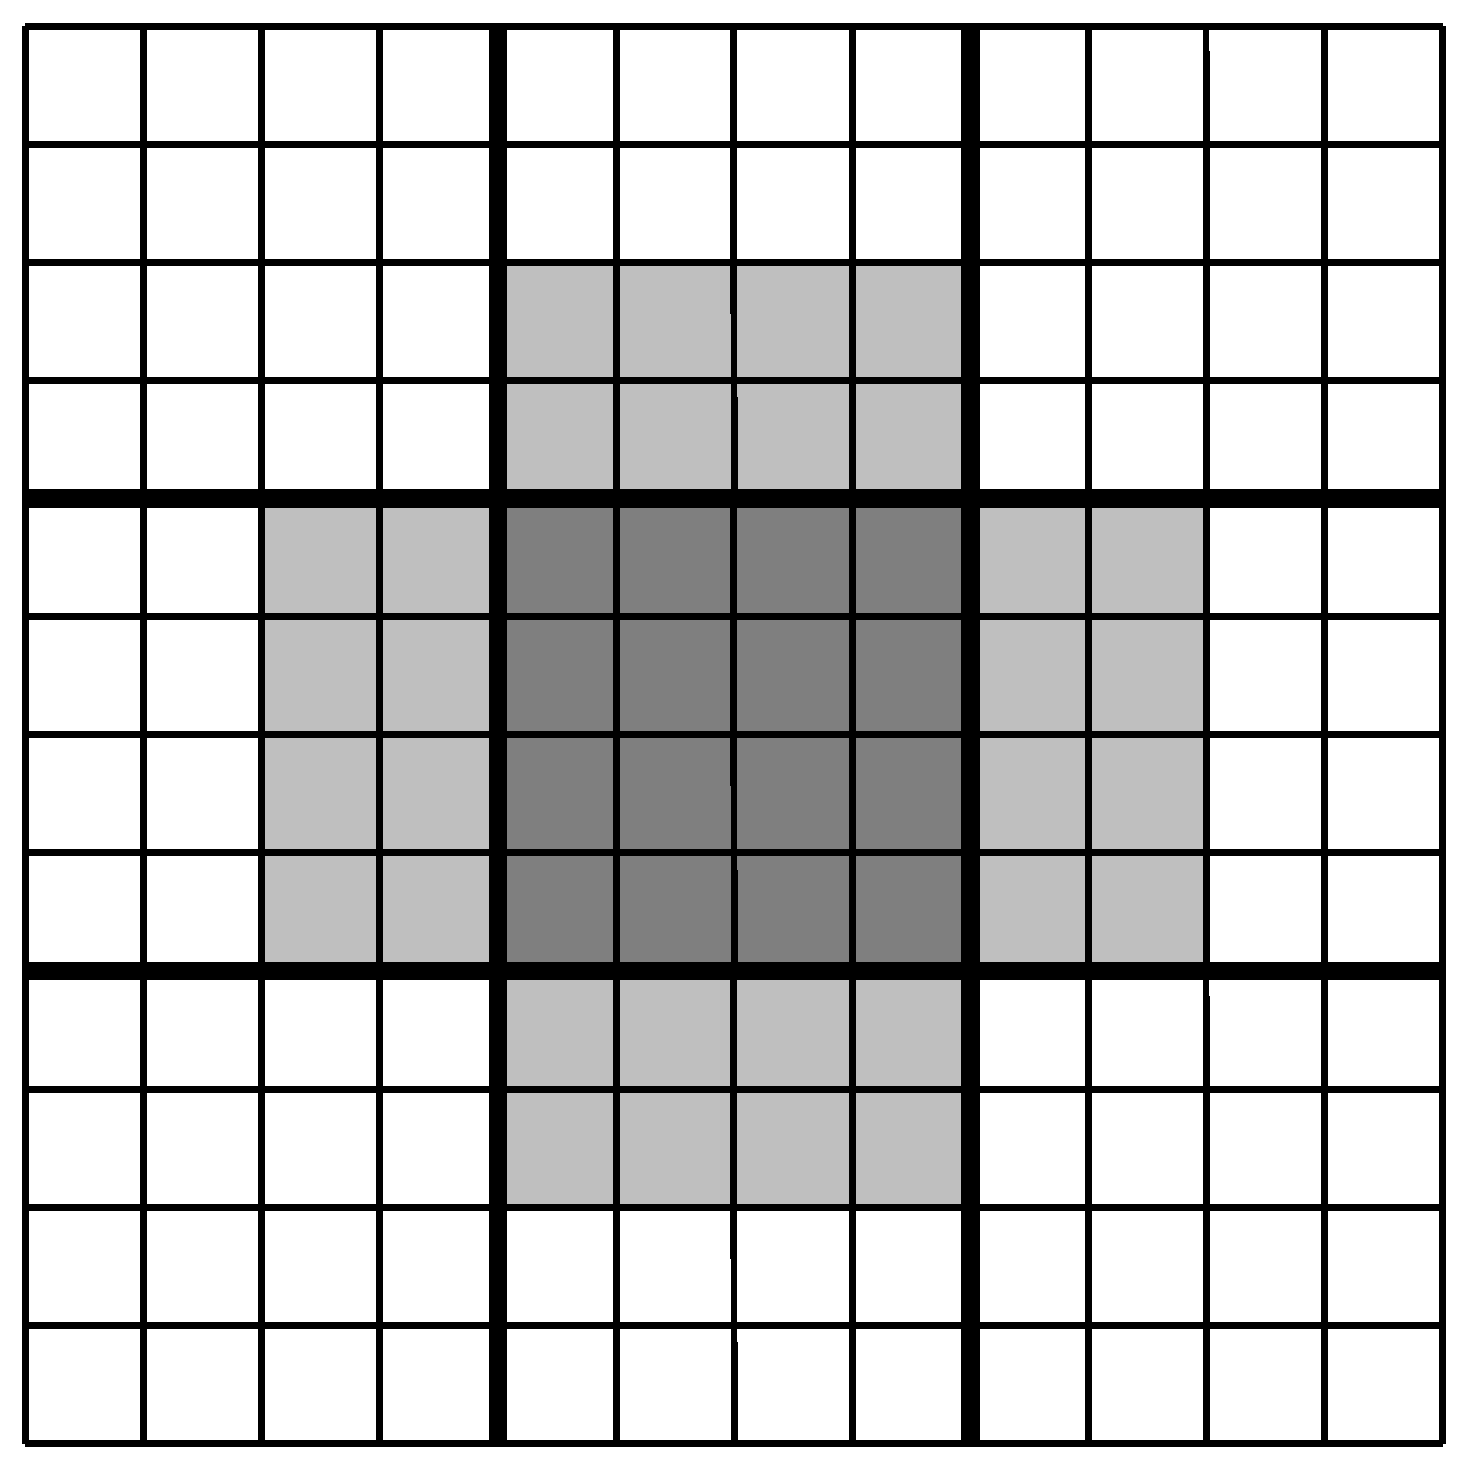
\includegraphics[width=90px]{gfx/diststencil}
 \caption{2D grid distributed over nine processes. A process needs some of its neighbor's surface points, to compute its own surface points.}
 \label{fig:diststencil}
\end{figure}

Applying a stencil operation on a grid involves all MPI processes. It is possible for an MPI process to compute most of the points in the sub-grid assigned to it. However, points near the surface of the sub-grid, \emph{surface points}, are dependent on remote points located in neighboring MPI processes. This dependency is illustrated in Figure \ref{fig:diststencil}.

The straightforward approach, and the one used in GPAW, for making remote points available, is to exchange the surface points between neighboring MPI processes before applying the stencil operation. The serialized communication pattern looks like this:
\begin{enumerate}
 \item Exchange surface points in the first dimension.
 \item Exchange surface points in the second dimension.
 \item Exchange surface points in the third dimension.
 \item Apply the stencil operation.
\end{enumerate}

\section{Optimizations}\label{section:opt}
In order to make GPAW run faster on the BGP, we have explored different optimizations. Optimizations, which have been beneficial, will be discussed in this section.

The most obvious optimization is to exchange surface elements simultaneously in all three dimensions by using the following non-blocking communication pattern:
\begin{enumerate}
 \item Initiate the exchange of surface points in all three dimensions.
 \item Wait for all exchanges to finish.
 \item Apply the stencil operation.
\end{enumerate}
The idea is to fully utilize the torus network in all six directions simultaneously, see Table \ref{tab:bgp}.

Another important performance aspect is how to map the distributed real-space grids onto the physical network topology. The 3D torus network is used for point-to-point communication in MPI, thus it is the network, we should attempt to map the distributed real-space grids onto. Since the grids have the same number of dimensions as the torus network, and since the stencil operation may use periodic boundary condition, a torus topology is a perfect match to our problem. However, the BGP requires a partition with 512 or more nodes to form a torus topology. A partition under 512 nodes can only form a mesh topology.

\subsection{Multiple real-space grids}
Double buffering and communication batching are two techniques which can improve the performance of the stencil operation. Both techniques requires multiple real-space grids but the stencil operation is typically applied on thousands of real-space grids.

\subsubsection{Double buffering}

\begin{figure}
 \centering
 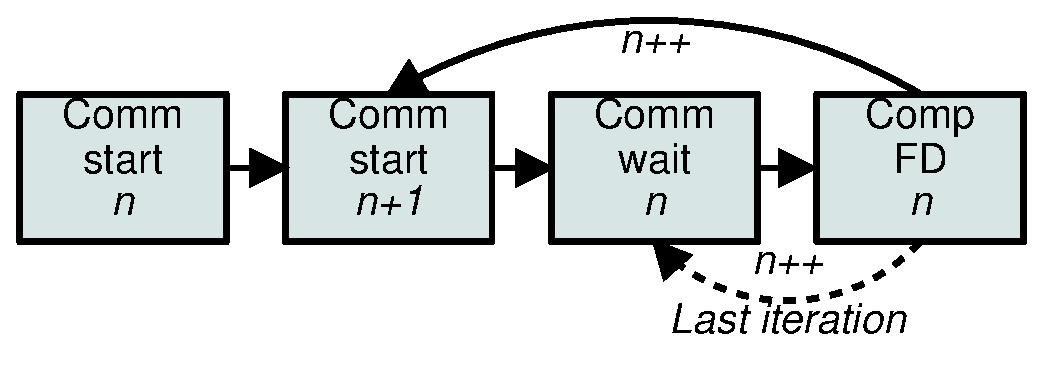
\includegraphics[width=200px]{gfx/commflow}
 \caption{Flow diagram illustrating double buffering. The $n$'th iteration is expressed with a $n$ and Comm and Comp stands for communication and computation, respectively. $n$++ is an iteration to $n$'s successor.}
 \label{fig:commflow}
\end{figure}

Double buffering is a technique that makes it possible to overlap communication and computation. The following communication pattern illustrates how (Figure \ref{fig:commflow}):
\begin{enumerate}
 \item Initiate the exchange of surface points in all three dimensions for the first grid.
 \item Initiate the exchange of surface points in all three dimensions for the second grid.
 \item Wait for all exchanges of the first grid to finish.
 \item Apply the stencil operation on the first grid.
 \item Initiate the exchange of surface points in all three dimensions for the third grid.
 \item Wait for all exchanges of the second grid to finish.
\end{enumerate}
The performance gain is dependent on the ability of the MPI library and the underlying hardware to process non-blocking send and receive calls. On the BGP, progress in non-blocking send and receive calls will be maintained by the DMA engine and increased performance is therefore expected.

\subsubsection{Batching}
An way to ensure critical packet size is to pack real-space grids into batches; inspired by the message size experiment (Figure \ref{fig:batchsize}).

Continuously dividing the grids between more and more MPI processes reduces the number of surface points in a single sub-grid. That is, at some point the amount of data send by a single MPI call will be reduced to a size in which the MPI overhead and network latency will dominate the communication overhead. The idea is to send a batch of surface points in each MPI call, instead of sending surface points, individually. This will reduce the communication overhead considerably, as the size of the sub-grids decreases. The number of grids packed together in this way, we call \emph{batch-size}.

When using double buffering, it is important to allow the CPUs to start computing as soon as possible. Combining a large batch-size with double buffering will therefore introduce a penalty as the initial surface points exchange cannot be hidden. One approach to minimize this penalty, is to increase the batch-size continuously in the initial stage. For instance a batch-size of 128 could be reduced to 64 in the initial exchange.

\section{Programming approaches}
Different approaches exist when combining threads and MPI. To preserve control we have chosen to handle the threading manually in pthread.

The following is a description of different programming approaches that we have investigated. Every programming approach except the \textbf{Flat original} uses the optimizations described in section \ref{section:opt}.

\begin{itemize}
 \item \textbf{Flat original} is the approach originally used in GPAW. It uses the BGP's virtual mode, where the four CPU-cores are treated as individual nodes, to utilize all four CPU-cores and it is therefore not necessary to modify anything to support the BGP architecture.

 \item \textbf{Flat optimized} is an optimized version of the original approach and just like the \textbf{Flat original} it uses the virtual mode.

 \item \textbf{Hybrid multiple} does not use the virtual mode. Instead, one hardware thread per CPU-core is spawned. Every thread handles its own inter-node communication. The node will distribute the real-space grids between its four CPU-cores, not by dividing the grids into smaller pieces but by assigning different grids to every CPU-core. Because of this no synchronization is needed until all grids are computed and the synchronization penalty is therefore constant. This way of exploiting multiple grids is the main advantage of this approach.

 \item \textbf{Hybrid master-only} also spawns one thread per CPU-core, but only one thread, the \emph{master thread}, handles inter-node communication. Since we have to synchronize between every grid-computation, each grid-computation will be divided between the four CPU-cores. The synchronization penalty thus become proportional to the number of grids. On the other hand, this approach does work in \texttt{SINGLE} MPI-mode and the overhead associated with \texttt{MULTIPLE} is therefore avoided.
\end{itemize}

\begin{figure}
 \centering
 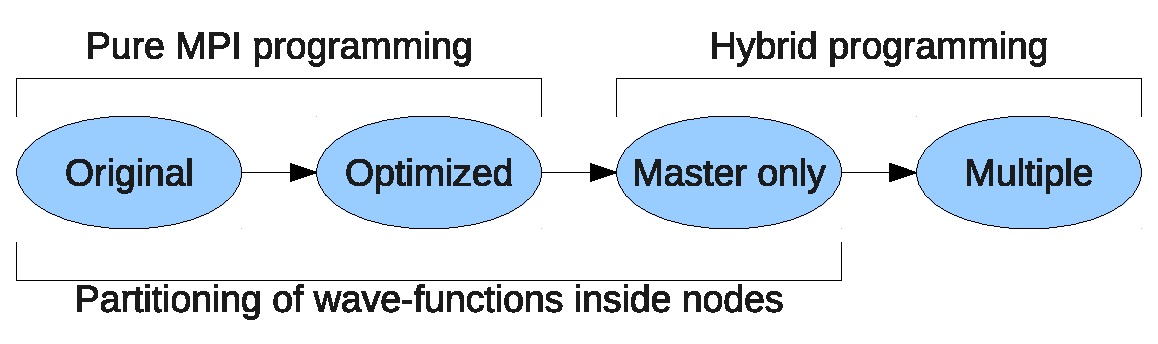
\includegraphics[width=\linewidth]{gfx/approaches}
 \caption{A illustrates of the connection between four programming approaches.}
 \label{fig:approaches}
\end{figure}

Figure \ref{fig:approaches} illustrates the connection between the four programming approaches -- from the original approach, in which pure MPI programming is used and the wave-functions are partitioned inside the nodes, to the hybrid approach where hybrid programming is used and the wave-functions are shared inside the nodes.


\section{Results}
A benchmark of each implementation has been executed on the Blue Gene/P. 16384 CPU-cores or 4096 nodes or 4 racks were made available to us. Every benchmark graph compares the different programming approaches of the stencil operation in GPAW and a periodic boundary condition is used in all cases.

Figure \ref{fig:speedup} is a classic speedup graph comparing every implemented approach with a sequential execution. It is a relatively small job containing only 32 real-space grids. But because of the memory demand, it is not possible to have more than 32 grids running on a single CPU-core.

The result clearly show that the best scaling and running time is obtained with \textbf{Flat optimized} and \textbf{Hybrid multiple} both using a batch-size of 8 grids. Since the job only consists of 32 grids a batch-size of 8 is the maximum if all four CPU-cores should be used. Another interesting observation is that the advantage of batching is greater in \textbf{Hybrid multiple} than in \textbf{Flat optimized}. This indicates that if a job consist of more grids, the \textbf{Hybrid multiple} approach may become faster than \textbf{Flat optimized}.

\subsection{Communication and Computation Profile}
The communication and computation profile becomes very important when scaling to a massive number of processes. As the number of MPI processes increases the communication time has a tendency to increase due to network congestion. It is therefore essential that all communication is spread evenly between the CPU-core and that the diversity of the communication and computation time is minimized. 

Figure \ref{fig:prof} is a profile of the \textbf{Hybrid multiple} approach executing on 1024 CPU-cores. It shows a distinct pattern in which the communication and the computation phase are aligned throughout the execution. From that it is evident that \textbf{Hybrid multiple} actually do execute in a fairly synchronized manner and no ripple effect of waiting processes is observed.


\begin{figure}
 \centering
 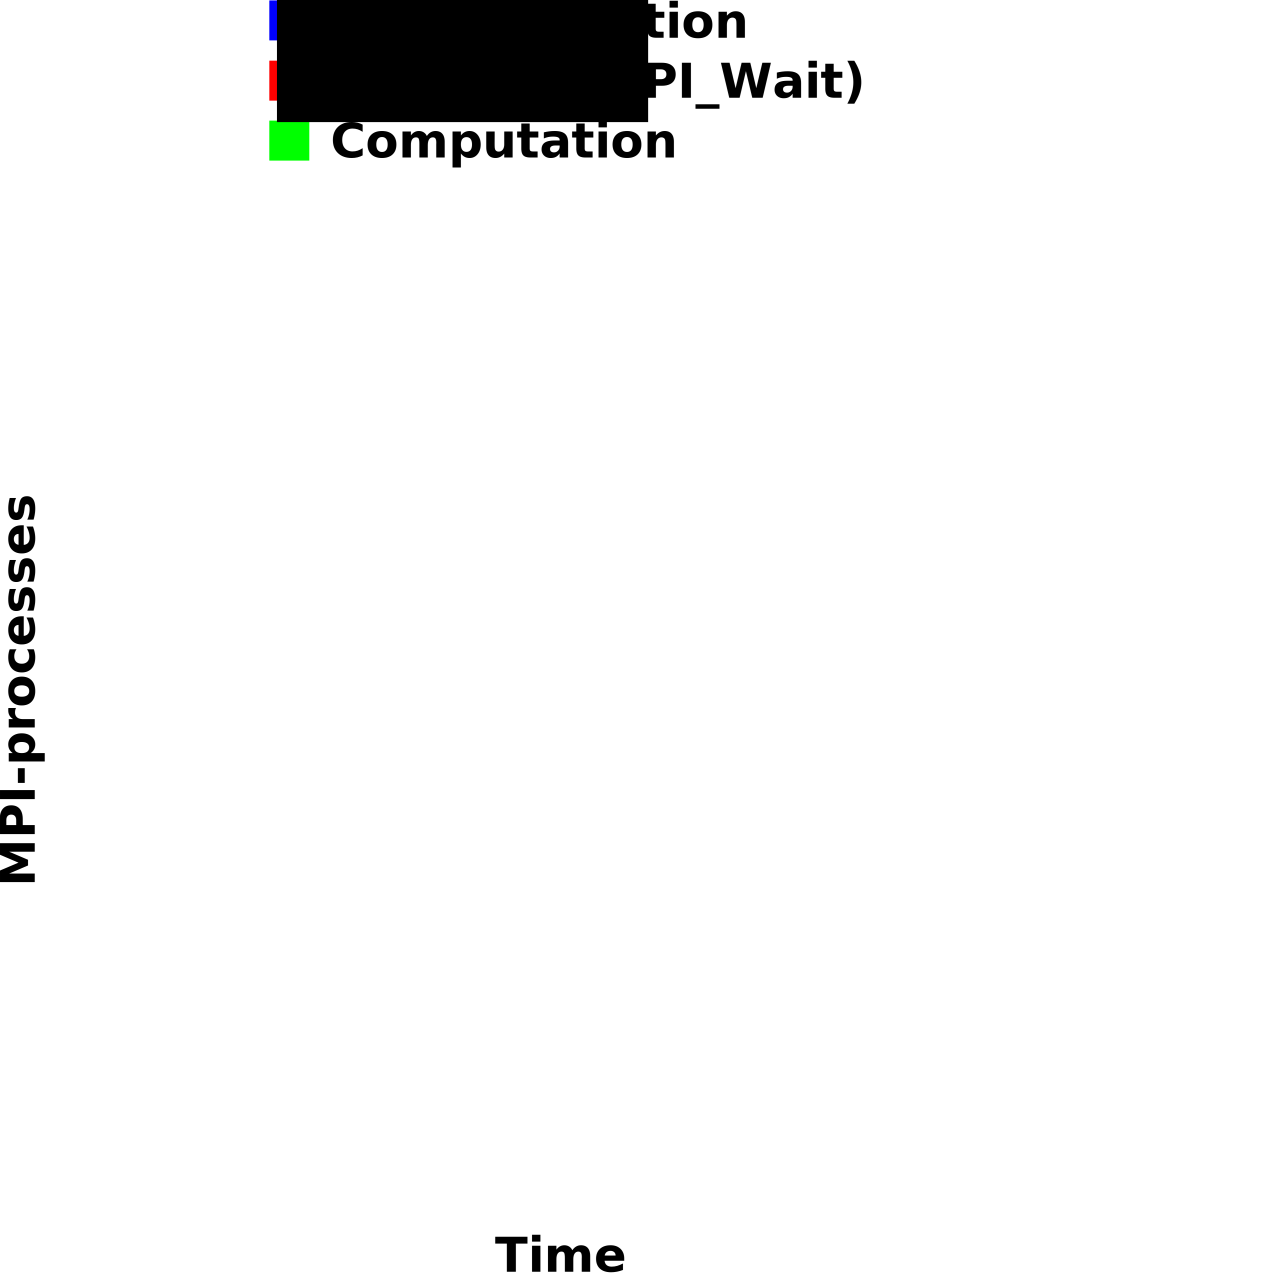
\includegraphics[width=\linewidth]{gfx/prof}
 \caption{Profile of the communication and computation pattern when computing 1024 real-space grids on 1024 CPU-cores and the \textbf{Hybrid multiple} approach is used. A line represents a MPI-process and the length of the line represents the progress of time.}
 \label{fig:prof}
\end{figure}


\subsection{Multiple real-space grids}
As the number of grids grow there is a corresponding linear growth in the computation required in the stencil operation. It is therefore possible to create a Gustafson graph by increasing the number of grids in the same rate as the number of CPU-cores (Figure \ref{fig:gustafson}). It is important to note that the required communication per node increases faster than the needed computation. This is due to the increased surface size associated with the additional partitioning of the grids. To illustrate this communication increase, the right graph in Figure \ref{fig:gustafson} shows the needed communication per node for \textbf{Flat optimized} and \textbf{Hybrid multiple} respectively.

If we, for example, look at a computation of a grid with a size of $192^3$ using 1024 nodes, the grid will either be divided between 1024 MPI processes when using \textbf{Hybrid multiple} or 4096 MPI process when using \textbf{Flat optimized}. \textbf{Flat optimized} needs to communicate approximately 140KB more data per node than \textbf{Hybrid multiple}. Note that this is only for a single real-space grid, the different will grow linearly with the number of grids in the computation.

At 512 CPU-cores \textbf{Hybrid multiple} is faster than \textbf{Flat optimized}. The main reason is the difference in the needed communication. \textbf{Flat optimized} divides the grids four times more than the \textbf{Hybrid multiple}. We did not see this effect in the speedup graph, Figure \ref{fig:speedup}, because of the small number of grids. Furthermore, \textbf{Hybrid multiple} is better to exploit an increase in grids because of the thread synchronization overhead. The overhead is small and constant, but since the total running time is very small for 32 grids (9 milliseconds with 2048 CPU-cores), the impact of the synchronization overhead is drastically reduced when the number of grids, and thereby the total running time, is increased.

To investigate the scalability of a large job with many real-space grids, we have made a scalability graph beginning at 1k CPU-cores, which allows for a 2816 grid job (Figure \ref{fig:scale}). Again \textbf{Hybrid multiple} has the best performance - going from 1k to 16k CPU-cores gives a speedup of approximately 12.5 where 16 would be linear but unobtainable due to the increase in the needed communication. If we compare the running time of \textbf{Hybrid multiple} with \textbf{Flat original}, we see a 94\% performance gain at 16384 CPU-cores.

%Again \textbf{Hybrid multiple} has the best performance - going from 1k to 16k CPU-cores gives a speedup of approximately 16.5 compared to \textbf{Flat original}. Comparing \textbf{Hybrid multiple} with itself, we have a speedup of 12 where 16 would be linear but unobtainable due to the increase in the needed communication.

To further investigate the performance difference between \textbf{Hybrid multiple} and \textbf{Flat optimized}, we have made a small experiment. We modifies \textbf{Flat optimized} to statically divide the real-space grids into four sub-groups. It is now possible for all four CPU-cores to work on its own sub-group and the real-space grids will be divided into the same level as in \textbf{Hybrid multiple}. The only difference between the two approaches is that \textbf{Flat optimized} uses the virtual mode in Blue Gene/P and \textbf{Hybrid multiple} uses threads.
It should be noted, however, that in a real GPAW computation this modification does not work, since GPAW requires that every MPI process gets the same subset of every real-space grid, see section \ref{section:GPAW_impl}.
The experiment is not included in any of the graphs since its performance is identical with the \textbf{Hybrid multiple}. Because of the identical performance, we find it reasonable to conclude that the level of real-space partitioning is the sole reason for the performance difference between \textbf{Hybrid multiple} and the non-modified \textbf{Flat optimized}.

\begin{figure*}
\centerline{
\mbox{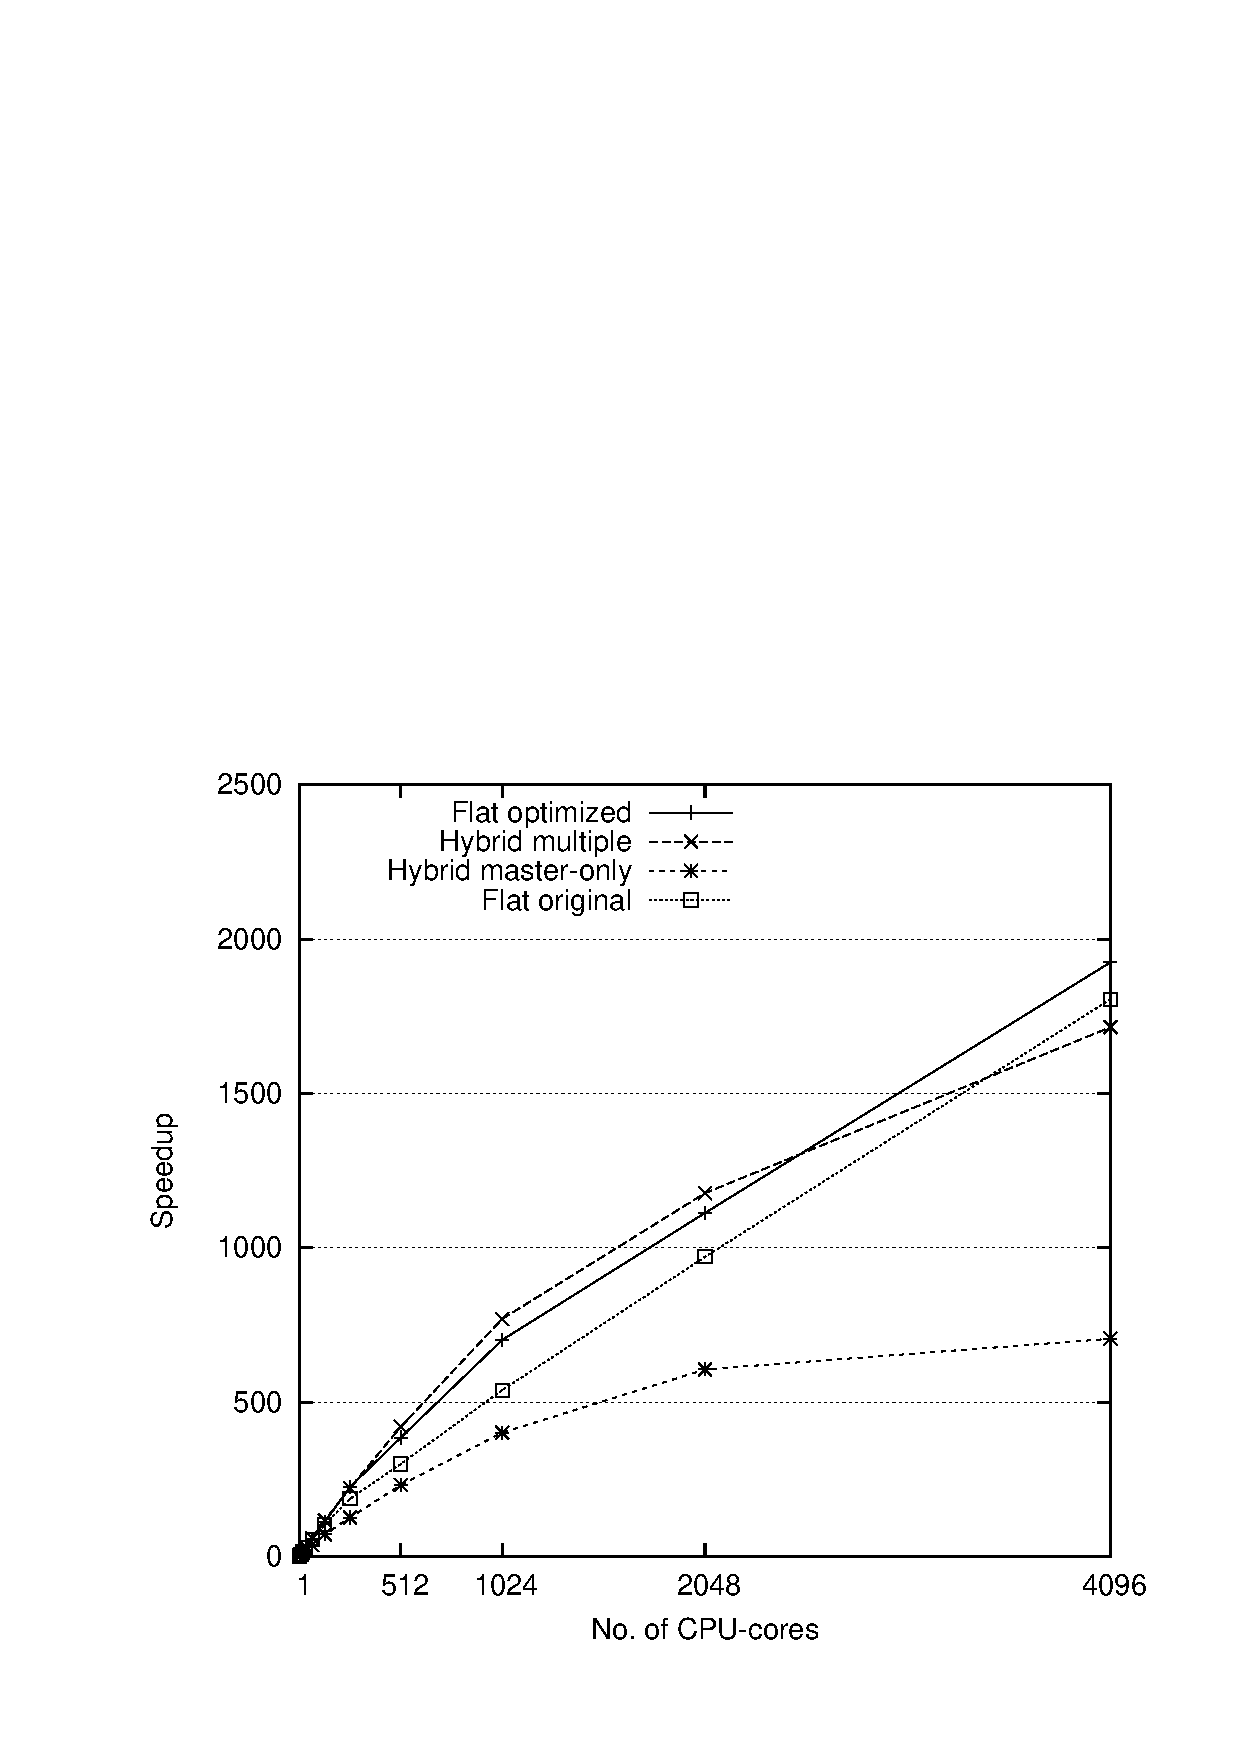
\includegraphics[width=250px]{gfx/fidi_speedup}}
\mbox{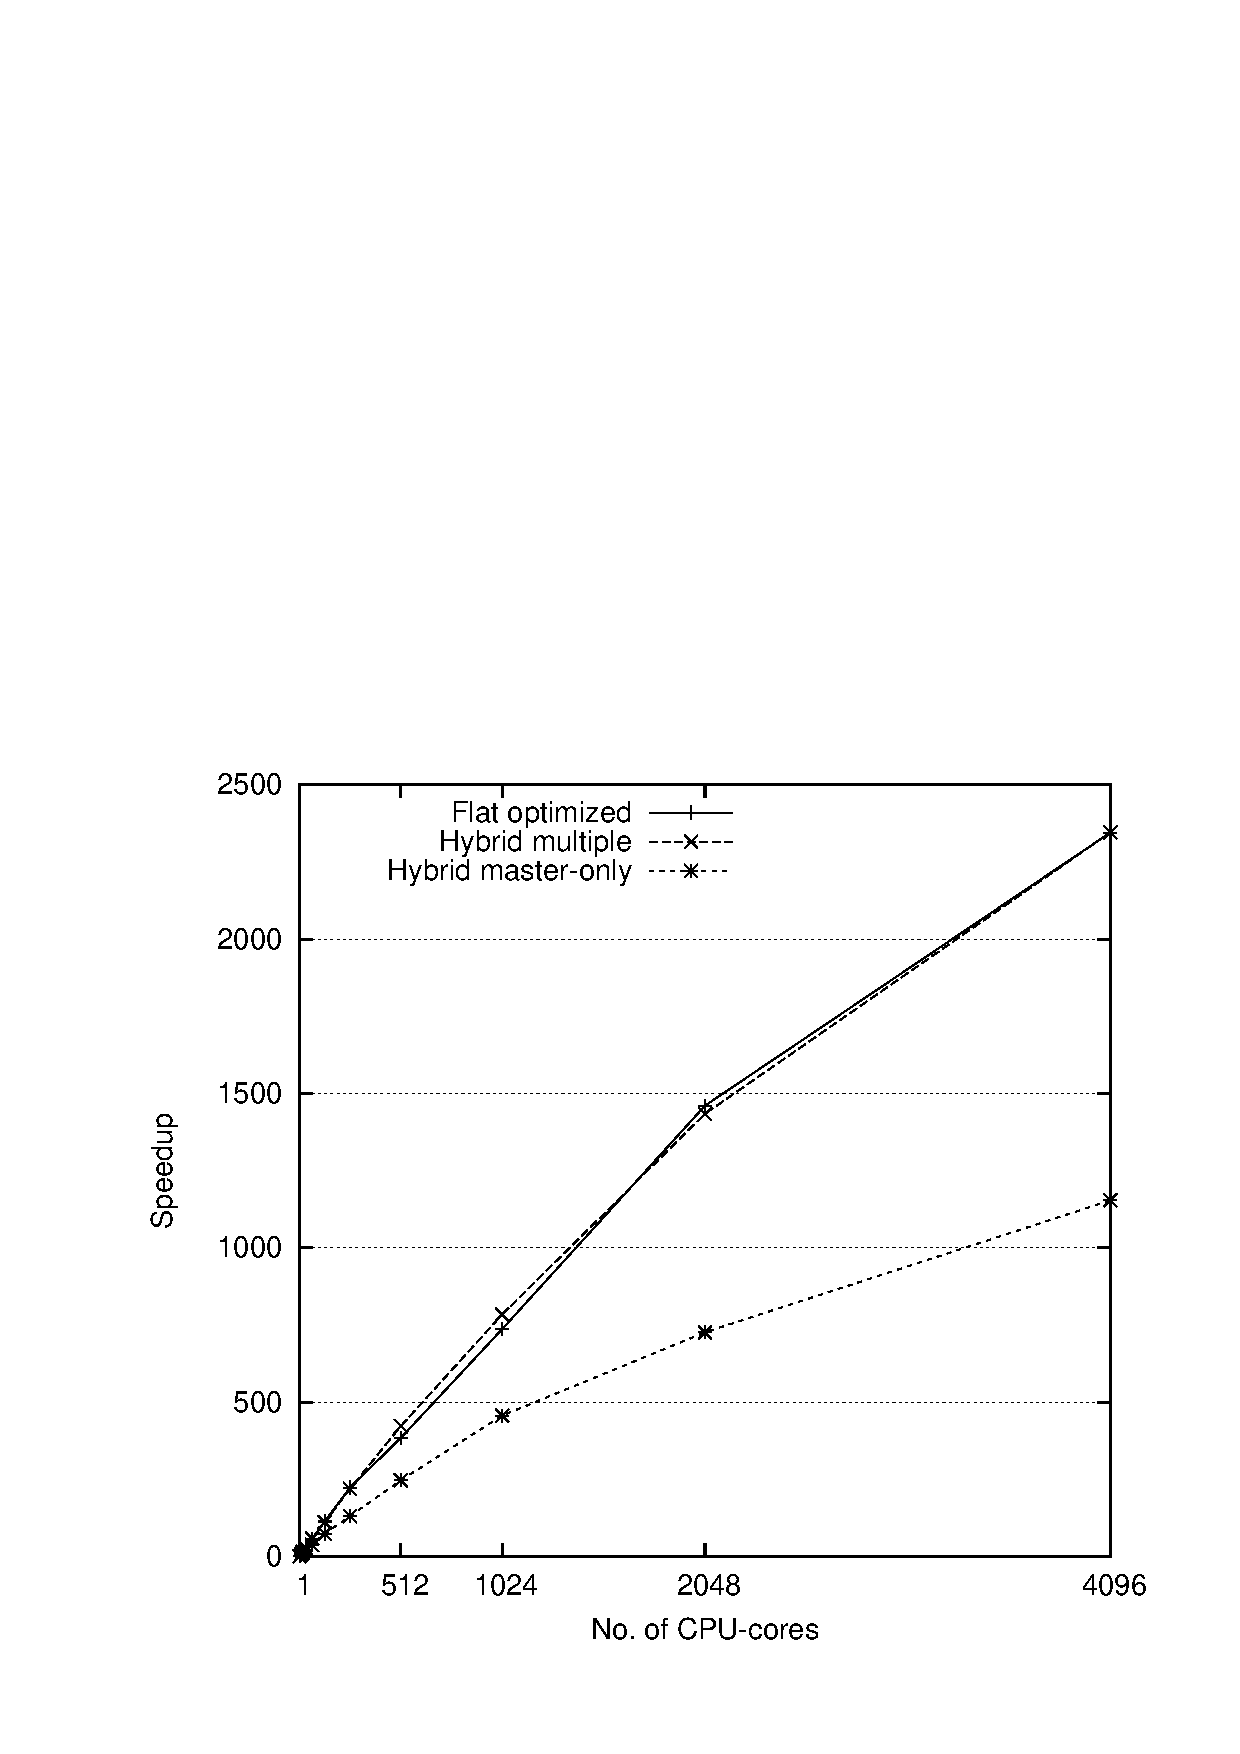
\includegraphics[width=250px]{gfx/fidi_batchspeedup}}
} 
 \caption{Speedup of the stencil operation. The job consist of only 32 real-space grids all with a size of $144^3$. In the left graph batching is disabled and in the right graph batching is enabled using a batch-size of 8.}
 \label{fig:speedup}
\end{figure*}

\begin{figure*}
\centerline{
\mbox{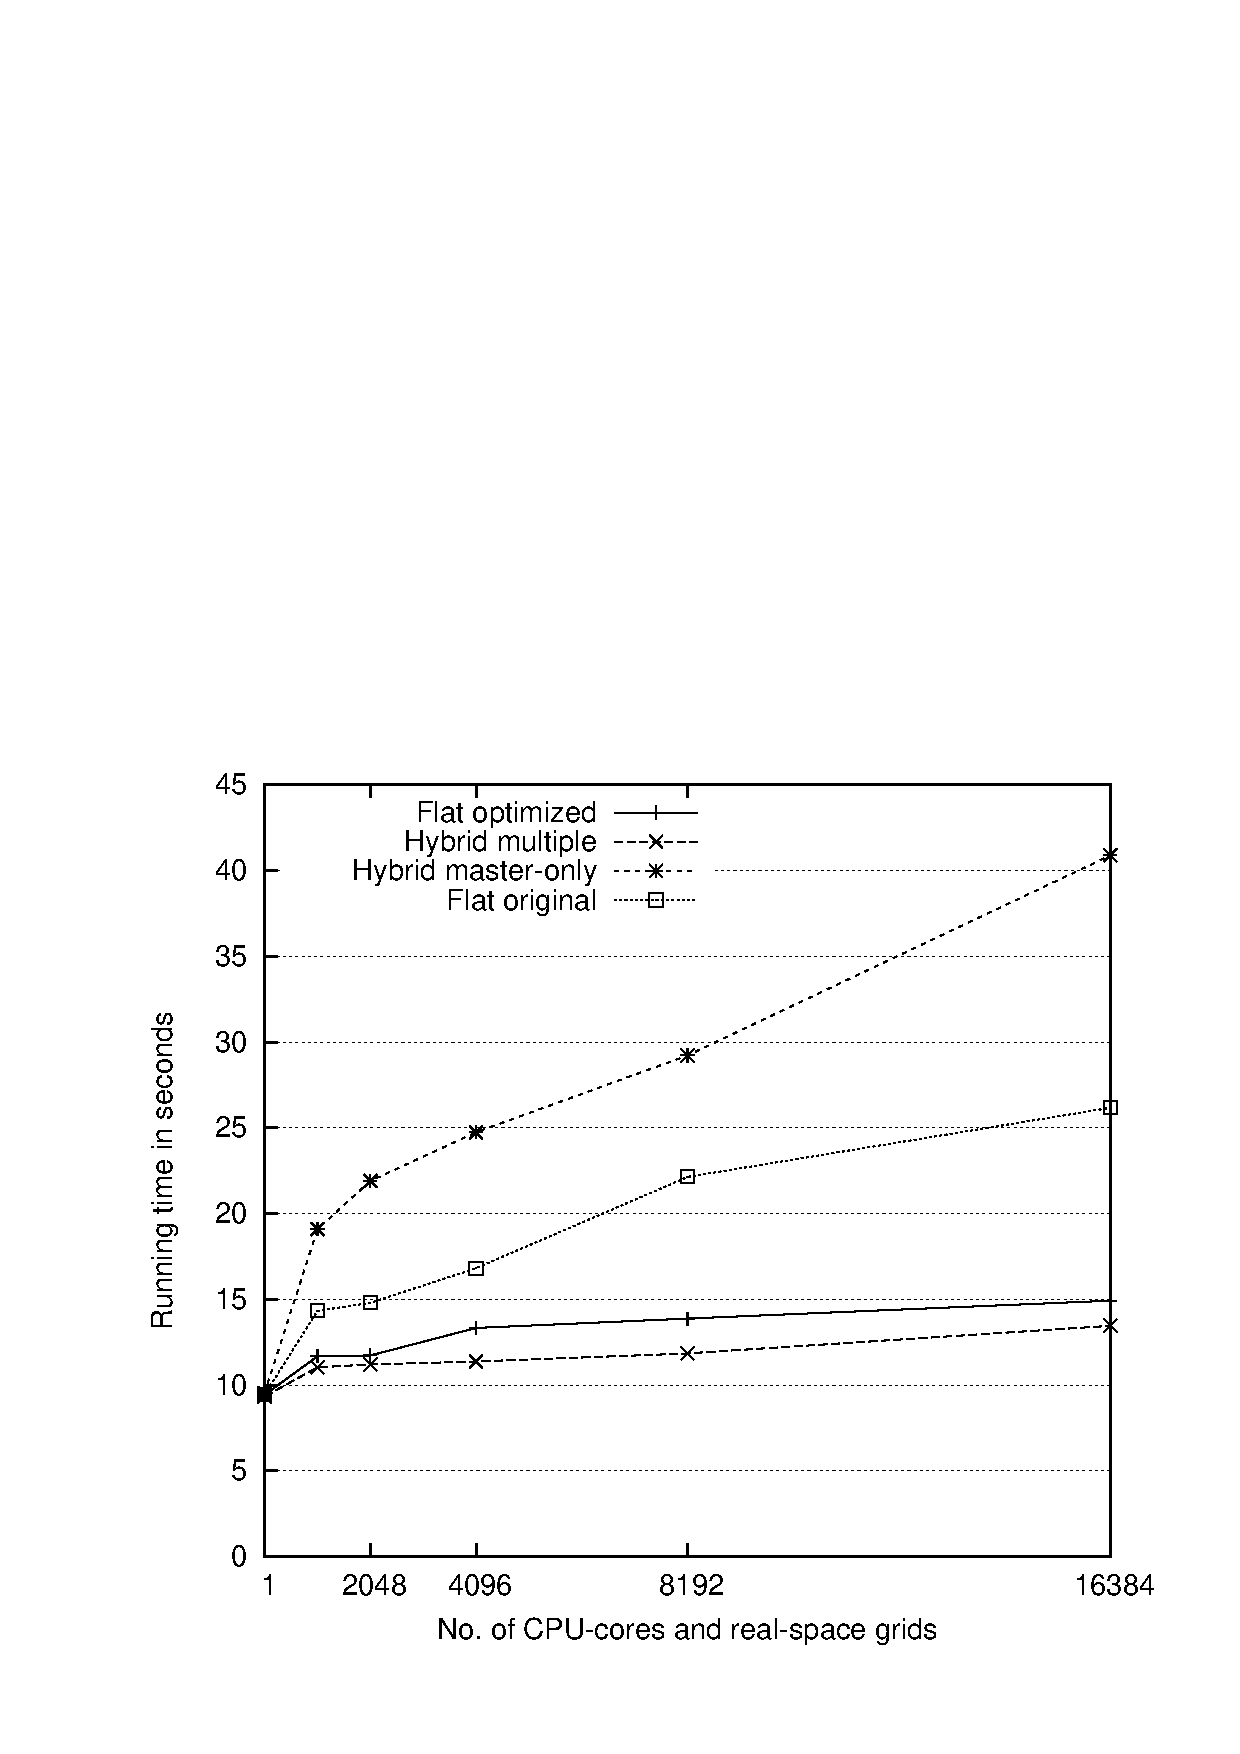
\includegraphics[width=250px]{gfx/fidi_gustavson}}
\mbox{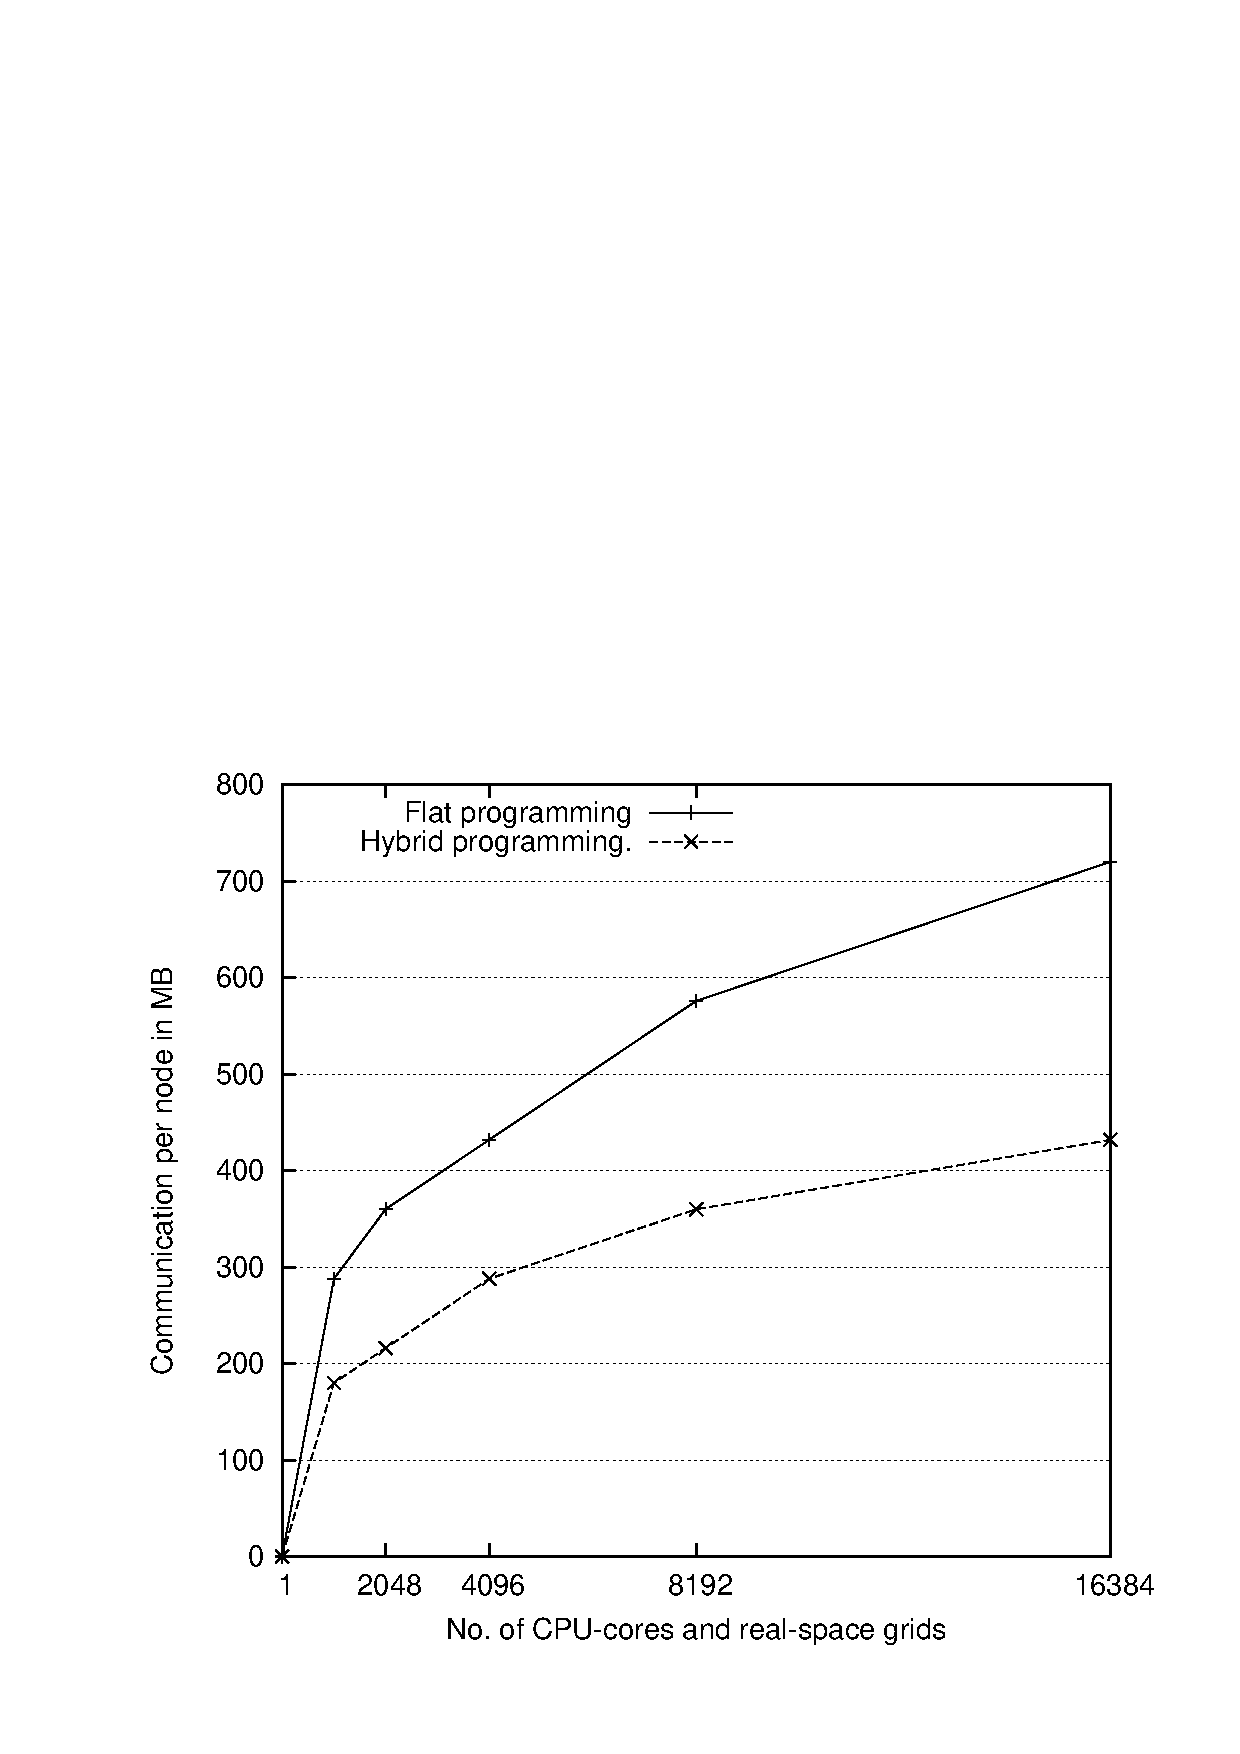
\includegraphics[width=250px]{gfx/fidi_gustavson_comm}}
} 
 \caption{Gustafson graphs showing the running time of the stencil operation and the needed inter-node communication when the number of real-space grids is increasing in the same rate as the number of CPU-cores - one grid per CPU-core. The left graph shows the running time and the right graph shows the needed inter-node communication. The grid size are $192^3$ and the best batch-size has been found for every number of CPU-cores. }
 \label{fig:gustafson}
\end{figure*}


\begin{figure*}
\centerline{
\mbox{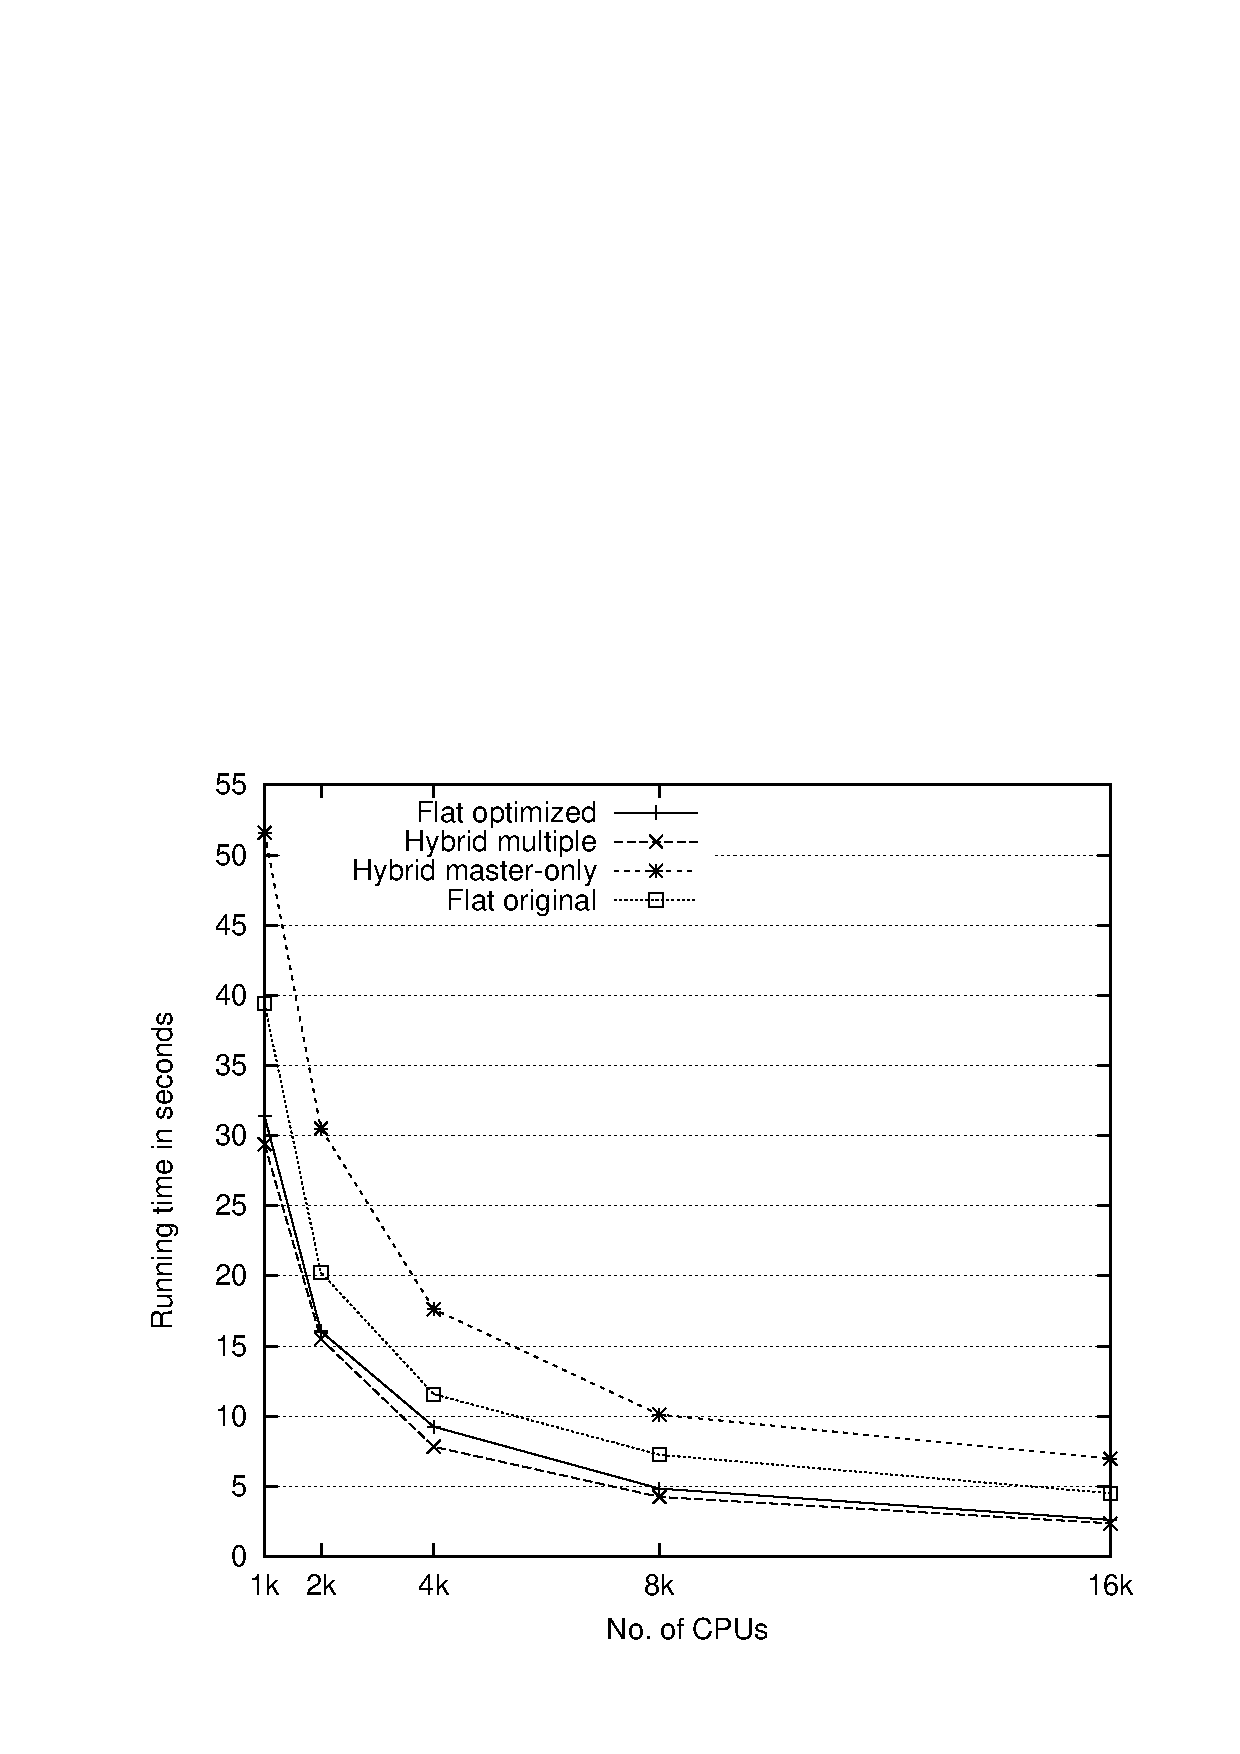
\includegraphics[width=250px]{gfx/fidi_scaleruntime}}
\mbox{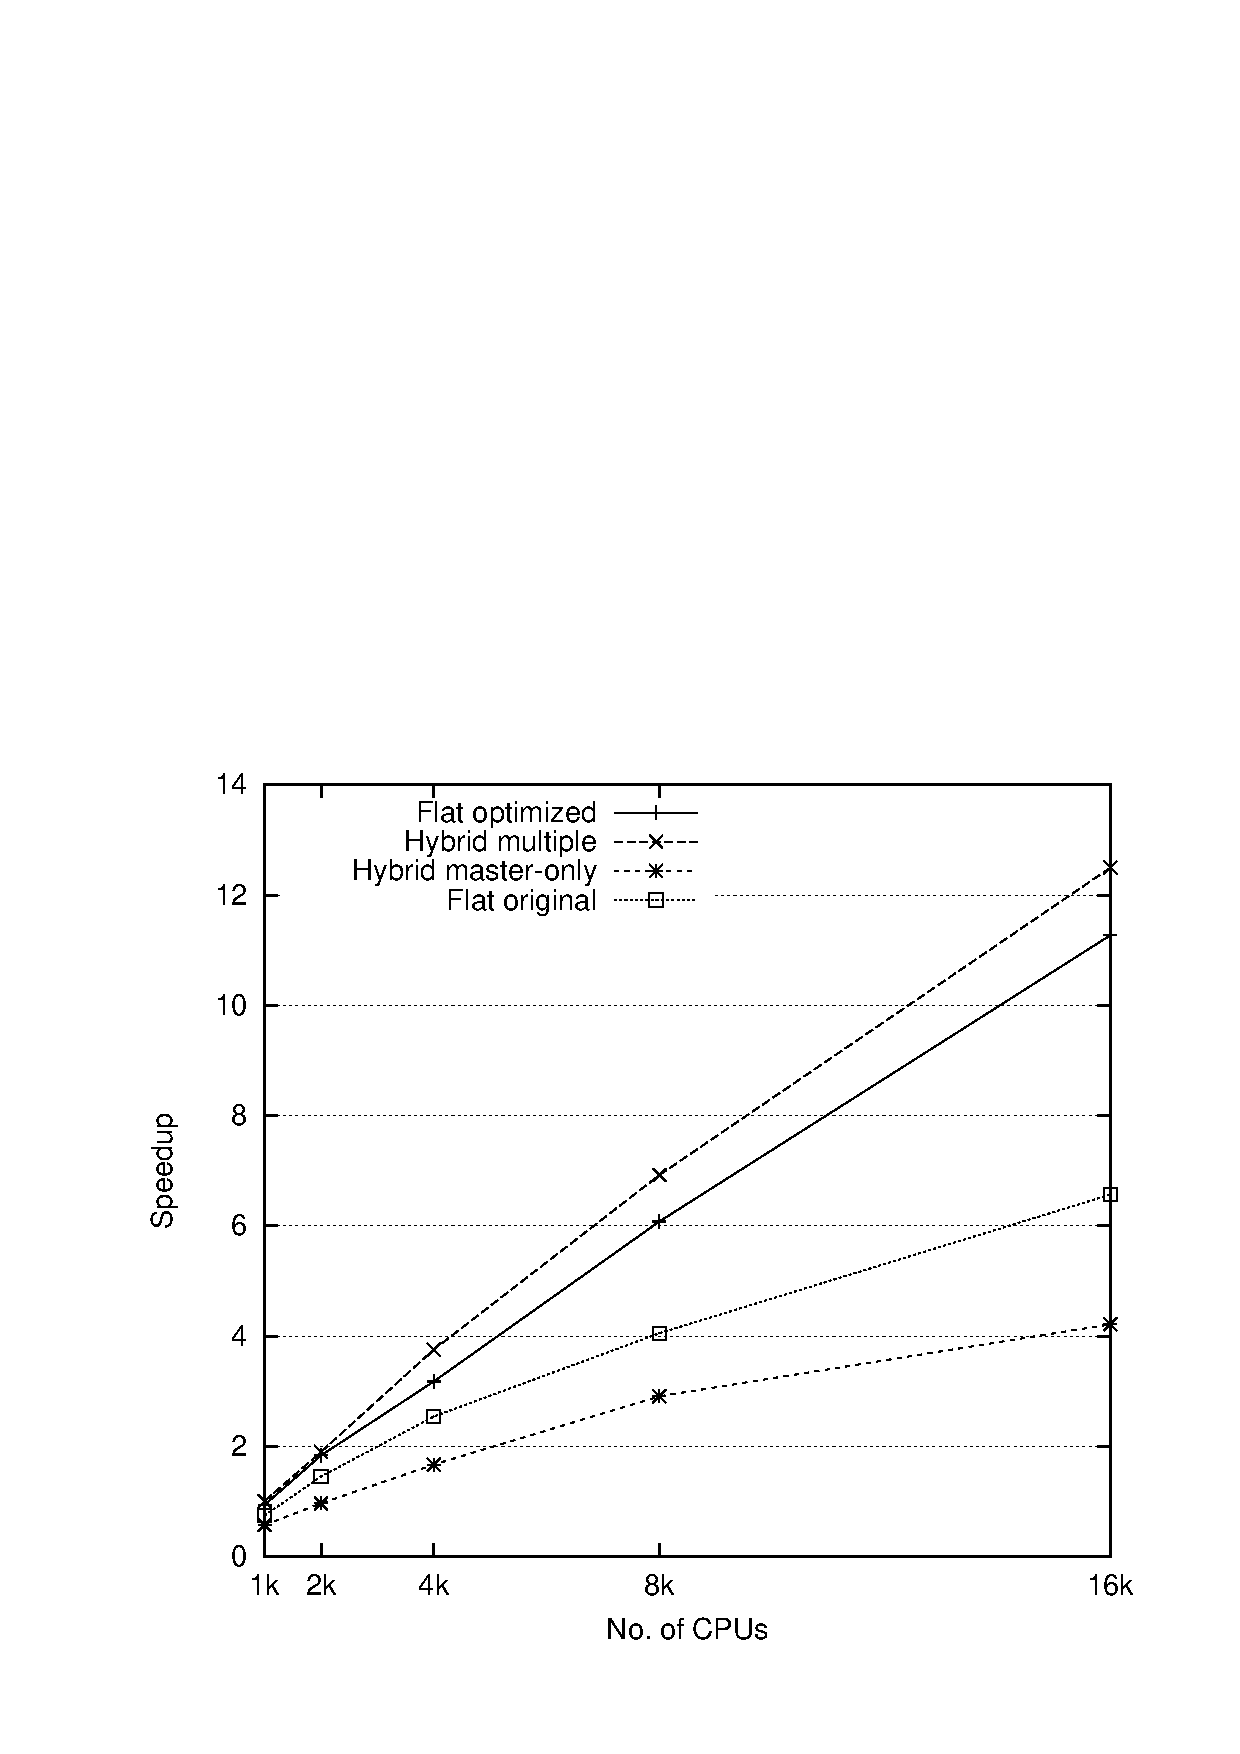
\includegraphics[width=250px]{gfx/fidi_scale}}
} 
 \caption{A scalability graph starting at 1024 CPU-cores running the stencil operation. In the left graph the running time of every approach is shown and in the right graph every approach is compared to the fastest approach on 1024 CPU-cores namely the \textbf{Hybrid multiple}. All jobs consists of 2816 real-space grids all size of $192^3$, and the best batch-size has been found for every number of CPU-cores.}
 \label{fig:scale}
\end{figure*}


\section{Conclusions}
Overall this work has managed to improve the performance of a domain specific stencil code when scaling to a very high degree of parallelism. The primary improvements are obtained through the introduction of asynchronous communication which, even in a well balanced system such as the Blue Gene, efficiently improves processor utilization. Furthermore, two hybrid programming approaches have been explored: the hybrid multiple and the master-only approach. 

The hybrid programming approach, in which inter-node communication is handled individually by every thread, has shown a positive impact on the performance. By allowing every thread to handle its own inter-node communication, the overhead for thread synchronization remains constant and the application becomes faster than the non-hybrid version.

On the other hand, the alternative hybrid programming approach, in which one thread handles the inter-node communication on behalf of all threads in the process, cannot compete with the non-hybrid version. That is explained by the overhead that is introduced by thread synchronization which grows proportional to the number of grids in the computation.

When comparing our fastest implementation compared to the original implementation, the hybrid programming approach combined with the latency-hiding techniques is 94\% faster at 16384 CPU-cores. Translated into utilization this means that CPU utilization grows from 36\% to 70\%.

While latency-hiding is the primary factor for the improvement we observe, the hybrid implementation is still 10\% faster than the non-hybrid approach.

\subsection{Further work}
Overall we are satisfied with the performance of the new implementation of the stencil operation, still a lot of work remains if the entire GPAW computation should utilize latency-hiding and hybrid programming. It may not be worth the hard work that is needed to rewrite most of GPAW, but it is our expectation that an overall performance gain as the one demonstrated in this work may be obtained for the application overall.

\section{Acknowledgments}
The authors would like to thank The Danish Agency for Science, Technology and Innovation and the GPAW team at the Technical University of Denmark in particular Jens J. Mortensen and Marcin Dulak. Furthermore we would like to thank Argonne National Laboratory for giving us access to the Blue Gene/P.


\bibliographystyle{model1b-num-names}
\bibliography{main}


\end{document}

